\chapter{O software desenvolvido \label{cap:software}}

Neste capítulo são apresentados aspectos práticos e construtivos do
software desenvolvido, indo desde uma descrição básica da funcionalidade
do sóftware, até alguns resultados práticos e caracteristicas da linguagem
de programação utilizada no projeto do software.

\section{Descrição do software}

    Este trabalho se baseia em um software, construido em linguagem Python
    e disponivel via \ac{WWW}. O software, batizado de \textbf{PIDSIM},
    possui os 14 processos industriais referenciais apresentados no capítulo
    \ref{cap:processos-referenciais} implementados, bem como diversos
    métodos numéricos para modelagem de sistemas (que serão discutidos no
    Anexo 1), métodos de identificação de sistemas (discutidos no capítulo
    \ref{cap:metodos-de-identificacao-e-sintonia}) e métodos de sintonia de
    controladores \acs{PID} (também discutidos no capítulo
    \ref{cap:metodos-de-identificacao-e-sintonia}).

    O software possui fins didáticos e foi construido visando facilitar a
    utilização por parte dos alunos durante as aulas ou durante o estudo em casa.
    Todas as tecnologias utilizadas são livres e estão disponíveis na internet,
    bem como o código-fonte dos modulos que compõem o software.

    Este software é desenvolvido desde 2009 e passou por grandes modificações
    desde então, até chegar ao resultado disponível hoje.

    Há uma instância pública do software rodando no seguinte endereço: \\
    \url{http://pidsim.rafaelmartins.eng.br}

    O código-fonte do software está disponível em repositórios do Sistema
    de Controle de Versão Mercurial \cite{Mercurial}: \\
    \url{http://hg.rafaelmartins.eng.br/pidsim/}

    O software está licenciado sob a licença \ac{GPL-2} \cite{GPL-2}, podendo ser redistribuido
    livremente, de acordo com os termos da licença.

\section{A linguagem Python}

    Durante a década passada, o Python \cite{Python} (uma linguagem linguagem interpretada
    de alto-nivel) tornou-se o padrão de fato para a pesquisa científica
    exploratória, interativa e voltada à computação \cite{5725235}.
    
    A linguagem Python é uma linguagem de alto-nível, orientada a objetos,
    amplamente utilizada atualmente. É uma linguagem de uso geral, sendo
    usada para os mais diversos fins, seja a criação de um \textit{website}
    ou uma aplicação pra desktop, ou para a criação de um aplicativo científico
    com calculos complexos.
    
    Python é uma linguagem interpretada, e pode ser usada interativamente.
    Algumas pessoas podem assumir que isso limita o seu uso - por exemplo,
    que uma linguagem interpretada possivelmente não será rápida o bastante
    para programação científica -, mas isto não é verdade \cite{4160249}.

\section{Arquitetura do software}

    Uma das características marcantes do software livre é a possibilidade de
    usuários trabalharem no código-fonte do software e adicionar as funcionalidades
    que desejar, porém isto se torna dificil se a arquitetura do software não tiver
    sido bem planejada.

    Levando se a facilidade de expansão em consideração, foi construida uma estrutura
    modular para o software, dividindo-o em pacotes individuais, e com o minimo
    possível de interdependência entre si.
    
    \begin{center}
        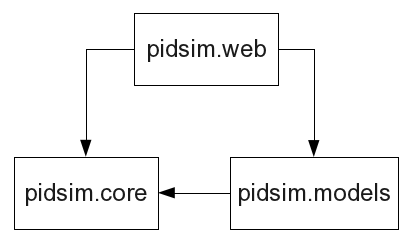
\includegraphics[width=0.6\textwidth]{imagens/cap4-pacotes.eps}
        \captionof{figure}{Dependencia entre os pacotes do software}
    \end{center}
    
    O software foi dividido em 3 pacotes Python:

    \begin{itemize}
        \item pidsim.core
        \item pidsim.models
        \item pidsim.web
    \end{itemize}

    Cada pacote tem sua funcionalidade especifica definida, e pode ser desenvolvido
    separadamente, facilitando bastante o desenvolvimento distribuido do software,
    que é uma das metas deste projeto.

    A adição e remoção de métodos é extremamente simples, facilitando as contribuições
    dos estudantes.

    Segue uma breve descrição de cada pacote Python que compõe o software:

    \subsection{pidsim.core}

        O pacote \textbf{pidsim.core} é o pacote principal do software, sendo responsável
        por toda a implementação básica, como os tipos de dados (com suporte a conversão
        de tipos e sobrecarga de operadores), os métodos numéricos, os algorítmos de controles,
        entre outras funcionalidades centrais do software.

        Este pacote foi implementado em Python puro, visando a possibilidade de utilização
        em sistemas onde não fosse possível compilar modulos Python escritos em linguagem C.
        Além disso, por se tratar de um projeto didático, não seria justificavel a utilização
        de um grande numero de bibliotecas prontas.

        \subsubsection{Tipos básicos de dados}

            Foram implementados os seguintes tipos básicos de dados:
        
            \begin{itemize}
                \item Polinômio
                \item Matriz
                \item Matriz Identidade
                \item Função de Transferência
                \item Espaço de Estados
            \end{itemize}

            Um ponto importante desta implementação de tipos de dados é a conversão de Função
            de Transferência para Espaco de Estados, que é vital para a discretização dos
            processos.

        \subsubsection{Métodos de discretização de processos}

            Foram implementados os seguintes métodos de discretização de processos:

            \begin{itemize}
                \item Euler
                \item RungeKutta de $2^a$ ordem
                \item RungeKutta de $3^a$ ordem
                \item RungeKutta de $4^a$ ordem
            \end{itemize}

            O estudante pode facilmente escolher qual dos métodos utilizar.

        \subsubsection{Aproximação de Padè}
            
            A implementação da aproximação de Padè criada é capaz de simular o tempo morto
            para alguns sistemas.

            Foi implementada a aproximação de Padè de $1^a$, $2^a$, $3^a$, $4^a$ e $5^a$ ordem.

        \subsubsection{Métodos de identificação de sistemas utilizando-se a curva de reação}
            
            Foram implementados os seguintes métodos de identificação dos sistemas utilizando-se
            a curva de reação:

            \begin{itemize}
                \item Alfaro
                \item Bröida
                \item Chen \& Yang
                \item Ho \textit{et al.}
                \item Smith
                \item Vitecková \textit{et al.}
            \end{itemize}

            Cada método possui suas características particulares, que já foram discutidas no capítulo
            \ref{cap:metodos-de-identificacao-e-sintonia}.

        \subsubsection{Métodos de sintonia para controladores \acs{PID}}
            
            Foram implementados os seguintes métodos de sintonia para controladores \acs{PID}:

            \begin{itemize}
                \item Ziegler \& Nichols
                \item Cohen \& Coon
                \item Chien \& Hrones \& Reswick 0\% de \textit{Overshoot}
                \item Chien \& Hrones \& Reswick 20\% de \textit{Overshoot}
            \end{itemize}

            Estes métodos também já foram discutidos no capítulo
            \ref{cap:metodos-de-identificacao-e-sintonia}.

        \subsection{pidsim.models}
            
            O pacote \textbf{pidsim.models} possui implementados os 14 processos referenciais
            discutidos no capítulo \ref{cap:processos-referenciais}.

            Cada processo é uma classe Python, com atributos específicos, como a expressão
            \LaTeX que representa o processo, um método Python que representa a função de
            transferencia básica do processo, uma lista de argumentos que esta função recebe,
            entre outros objetos necessários ao uso dos processos pela interface Web, ou qualquer
            outra interface que venha a ser desenvolvida.

        \subsection{pidsim.web}
            
            O pacote \textbf{pidsim.web} implementa a interface web, desenvolvida utilizando-se
            o \textit{framework web} \textbf{Flask}, que é responsavel pela geração das páginas
            WEB do software e o toolkit de plotagem de gráficos \textbf{Matplotlib}, que é
            responsável pela geração dos gráficos.

            Apesar da facilidade em se implementar interfaces para o software, devido à arquitetura
            implementada, apenas a interface web está disponível no momento.

\section{A interface WEB}

    A interface do software com o usuario é feita através da Internet, utilizando-se um aplicativo Web,
    desenvolvido com o \textit{framework web} \textbf{Flask}.

    Uma imagem com a tela inicial do software pode ser vista abaixo:
    
    \begin{center}
        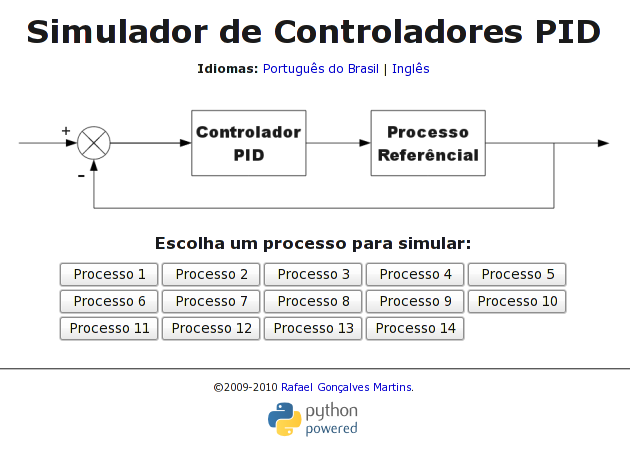
\includegraphics[width=0.8\textwidth]{imagens/cap4-pidsim_home.eps}
        \captionof{figure}{Tela inicial do software}
    \end{center}

    O software possui suporte a internacionalização. Utilizando se o pacote Python Babel. Atualmente está
    implementado o suporte ao Inglês e ao Português.
    
    \subsection{Exemplo - Processo de pólos múltiplos e iguais}
    
        O seguinte exemplo ilustra as funcionalidades disponíveis no software,
        utilizando o processo de pólos múltiplos e iguais como caso de uso.
        
        Segue a tela inicial do software, após selecionado o processo de
        pólos múltiplos e iguais (processo 5).
        
        \begin{center}
            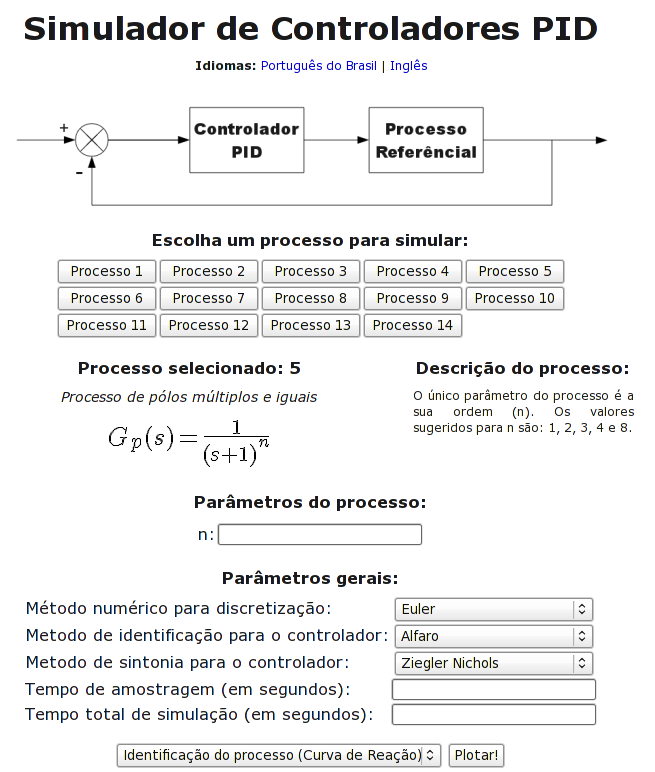
\includegraphics[width=0.8\textwidth]{imagens/cap4-model5-inicio.eps}
            \captionof{figure}{Tela inicial do processo de pólos múltiplos e iguais}
        \end{center}
        
        Para este exemplo, serão utilizados os seguintes valores de parâmetros:
        
        \begin{itemize}
            \item $n = 4$ - Processo de quarta ordem
            \item Método numérico para discretização: Runge-Kutta de quarta ordem
            \item Método de identificação para o controlador: Smith
            \item Método de sintonia para o controlador: Ziegler-Nichols
            \item Tempo de amostragem = 0.01s
            \item Tempo total = 20s
        \end{itemize}
        
        Um gráfico com estes parâmetros possuirá 2 mil pontos.
        
        O formulário preenchido pode ser visto na imagem abaixo.
        
        \begin{center}
            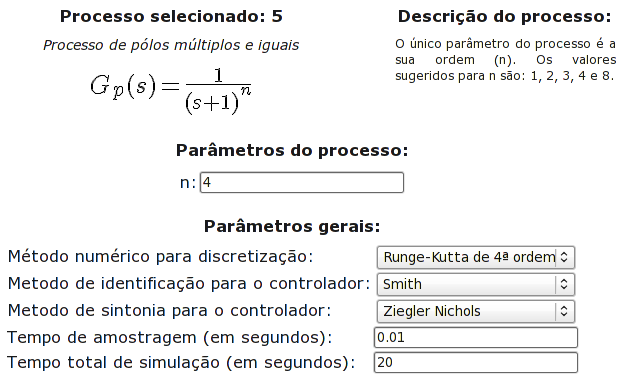
\includegraphics[width=0.8\textwidth]{imagens/cap4-model5-valores.eps}
            \captionof{figure}{Valores de parâmetros utilizados para a simulação de exemplo}
        \end{center}
        
        Após configurar os parâmetros, e clicar no botão "Plotar!", o software
        irá realizar a identificação do sistema. A figura abaixo representa o
        gráfico da identificação.
        
        \begin{center}
            \includegraphics[width=0.8\textwidth]{imagens/cap4_model5_1.eps}
            \captionof{figure}{Gráfico da identificação do processo de exemplo}
        \end{center}
        
        Para os parâmetros selecionados, os ganhos identificados para o
        controlador são: $kp=1.6$; $ki=0.4$ e $kd=1.5$.
        
        Após identificado o processo, é possível simular o controlador em
        operação, utilizando-se o menu que fica ao lado do botão "Plotar!".
        Vide gráfico resultante na figura abaixo.

        \begin{center}
            \includegraphics[width=0.8\textwidth]{imagens/cap4_model5_2.eps}
            \captionof{figure}{Gráfico da simulação do controlador para o processo de exemplo}
        \end{center}
        
        É possivel também alterar os valores dos ganhos $kp$, $ki$ e $kd$ manualmente.
        Este exemplo utilizará os ganhos: $kp=2.0$; $ki=0.9$ e $kd=1.4$,
        conforme a figura a seguir.
        
        \begin{center}
            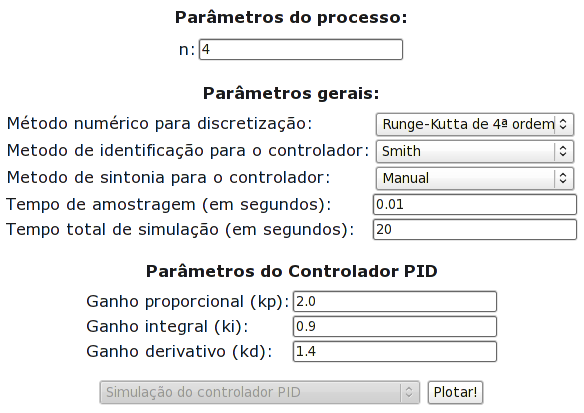
\includegraphics[width=0.8\textwidth]{imagens/cap4-model5-valores_manual.eps}
            \captionof{figure}{Valores dos ganhos do controlador para o processo de exemplo, escolhidos manualmente}
        \end{center}
        
        Executando a simulação para o controlador com os novos ganhos, escolhidos manualmente
        obtemos o seguinte gráfico:
        
        \begin{center}
            \includegraphics[width=0.8\textwidth]{imagens/cap4_model5_3.eps}
            \captionof{figure}{Gráfico da simulação do controlador para o processo de exemplo, com ganhos escolhidos manualmente}
        \end{center}
        
        Com todos estes dados e gráficos, o estudante será capaz de avaliar o desempenho
        do controlador, de acordo com os ganhos e métodos que desejar, até obter um
        controlador bem sintonizado.

\section{Conclusões parciais}

    Do desenvolvimento deste software, conclui-se que soluções em software livre
    para o estudo da engenharia são plenamente factíveis, e que proporcionam, tanto
    aos desenvolvedores quanto aos usuários finais, um grande aprendizado da teoria
    utilizada na implementação do mesmo.

    Da utilização deste software, conclui-se que existe uma enorme gama de variáveis
    envolvidas na sintonia de um controlador \acs{PID}, e que um simulador com as
    caracteristicas do mesmo é uma ferramenta importante para estudo.
